\chapter{Grundlagen}
\section{Laserlichtschneiden}

Beim Laserlichtschneiden wird ein fokussierter Laserstrahl auf die Werkstückoberfläche gerichtet. Das Material schmilzt lokal auf und wird mit einem zugeführten Gas aus dem Schnittspalt ausgeblasen. So entsteht eine schmale, definierte Trennfuge. Die grundlegenden Begriffe und Kenngrößen (z.\,B.\ Strahlleistung, Strahlqualität, Fokuslage) sind in \parencite{ISO11145-2018} beschrieben.

In der Produktion kommen vor allem Faser- und Scheibenlaser zum Einsatz. CO\textsubscript{2}-Laser werden seltener verwendet. Faser- und Scheibenlaser erlauben hohe Energiedichten im Brennfleck und damit hohe Schnittgeschwindigkeiten, besonders bei dünnen bis mittleren Blechdicken. Die Wahl des Prozessgases beeinflusst Schnittqualität und Kantenfarbe. Beim Schneiden mit Stickstoff bildet sich kaum Oxid an der Schnittkante, die Kante bleibt hell und metallisch. Das ist vorteilhaft, weil in der Regel weniger Nacharbeit erforderlich ist, wie z.B dem Nachbürsten der Kante, so dass wieder eine metalische Oberfläche zu sehen ist. Beim Schneiden mit Sauerstoff reagiert das Material mit dem Gas und somit entsteht eine dunkle Oxidschicht, die die Kante verfärbt. Der Prozess kann zwar schneller sein, führt aber demanch zu zusätzlicher Nacharbeit, wenn eine helle und einwandfreie Kante gefordert ist.

Die wichtigsten Einstellgrößen dieser sind die Laserleistung, Schnittgeschwindigkeit, Fokuslage und Gasdruck. Eine höhere Leistung erlaubt höhere Geschwindigkeit, bis die Qualitätsgrenzen erreicht sind. Eine unpassende Fokuslage führt schnell zu Grat oder unvollständigem Materialaustrag. Der Gasdruck muss so gewählt werden, dass die Schmelze zuverlässig aus dem Schnittspalt entfernt wird, ohne die Kante aufzurauen. Für die Bewertung der Schnittqualität sind u.\,a.\ Grat und Rauheit relevant. ISO~9013 fasst hierfür Klassen und Toleranzen zusammen \parencite{ISO9013-2017}.

Für Edelstahl gelten gegenüber Baustahl angepasste Einstellungen. Gründe sind unter anderem eine höhere Reflexion und eine geringere Wärmeabfuhr. In der Praxis bedeutet das, dass die Leistung und die Fokuslage sorgfältig abgestimmt werden müssen. Die Geschwindigkeit muss demnach passend gewählt werden. Als Prozessgas wird meistens Stickstoff eingesetzt, um eine helle Kante und geringen Grat zu erreichen.

\section{Grat und Rauheit eines Blechteils}

\label{sec:grat-rauheit}

Grat und Rauheit sind zentrale Merkmale der Schnittkante. Der Grat entsteht als aufgeworfener Materialüberschuss an der Unterkante. Er entsteht durch unvollständigen Schmelzaustrag oder durch Wiederanbacken von Schmelze im Schnittspalt. Die Rauheit beschreibt die feinen Höhenabweichungen der Schnittfläche entlang eines Profils. Für die Begriffe und Messregeln gelten die Definitionen in \parencite{ISO11145-2018} und die Qualitätsklassifikation thermischer Schnitte in \parencite{ISO9013-2017}. Für die geometrischen Rauheitskenngrößen wird nach ISO 4287 gemessen und ausgewertet.

\textbf{Rauheit.} Ein Rauheitsprofil \(z(x)\) entsteht nach Abtrennung von Form und Welligkeit über die festgelegte Grenzfrequenz. Der arithmetische Mittenrauwert \(R_a\) ist das Mittel der Beträge der Profilabweichung über die Auswertelänge \(L\)
\[
R_a=\frac{1}{L}\int_{0}^{L}\lvert z(x)\rvert\,\mathrm{d}x
\]
und in diskreter Form für \(n\) Stützstellen
\[
R_a=\frac{1}{n}\sum_{i=1}^{n}\lvert z_i\rvert\;.
\]
Häufig wird zusätzlich die mittlere Rautiefe \(R_z\) angegeben. Dafür wird die Auswertelänge in fünf Teilstücke zerlegt. In jedem Teilstück wird die Differenz zwischen höchstem Profilpunkt und tiefstem Profilpunkt gebildet. \(R_z\) ist das arithmetische Mittel dieser fünf Werte. \parencite{ISO9013-2017}

Die Grathöhe \(h_b\) wird als maximale positive Auslenkung des Profils im Bereich der unteren Schnittkante gemessen. Grundlage ist ein Profil senkrecht zur Schnittkante oder ein entlang der Kante geführtes Profil, das aus einer Punktwolke oder einem Tastschnitt abgeleitet wird. Neben der Höhe können Breite und Form des Grates beschrieben werden. Für Abnahme und Zeichnungseintrag wird die Zuordnung zu Qualitätsklassen nach \parencite{ISO9013-2017} verwendet.

Edelstahl besitzt eine geringere Wärmeleitfähigkeit und eine höhere Reflexion als Baustahl. Dadurch konzentriert sich die Eingangsenergie stärker in der Schnittzone. Die Schmelze bleibt zäher und fließt schwerer ab. Das begünstigt eine zackige Gratmorphologie und erhöht die Streuung der lokalen Rauheit. Beim Schneiden von Baustahl ist der Grat oft gleichmäßiger. Der Einsatz von Stickstoff unterstützt helle Kanten ohne Oxid und erleichtert die Nachbearbeitung. Sauerstoff kann höhere Vorschübe ermöglichen, führt aber zu einer dunklen Oxidschicht, die optisch auffällt und oft entfernt werden muss. Unabhängig vom Werkstoff wirken Leistung, Fokuslage, Schnittgeschwindigkeit, Gasdruck und Düsenabstand zusammen. Zu geringe Leistung oder zu hohe Geschwindigkeit erhöhen die Wahrscheinlichkeit von Grat und unruhigen Schnittflächen. Ein unpassender Fokus oder ein zu niedriger Gasdruck verschlechtert den Schmelzaustrag und erhöht die Rauheit.

In der Praxis wird das Profil aus einer 3D-Punktwolke oder aus Bilddaten erzeugt. Aus diesem Profil werden \(R_a\) und \(R_z\) berechnet. Die Grathöhe wird aus demselben Profil im Randbereich bestimmt. Eine klare Kennzeichnung der Messstellen und der Parameter sorgt dafür, dass Werte zwischen Werkstücken und Dicken vergleichbar bleiben.

In Abbildung~\ref{fig:roughness-profile} ist das Prinzip der Rauheitsbestimmung schematisch dargestellt. Die rote Linie zeigt die Bezugslinie. \(z_i\) sind die Profilwerte und \(X_{s}\) markiert eine Teilstrecke für die Auswertung von Kenngrößen wie \(R_z\).

\begin{figure}[htbp]
  \centering
  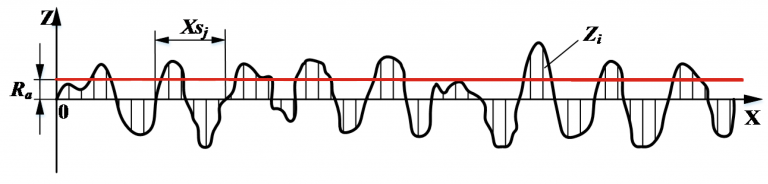
\includegraphics[width=\linewidth]{burr_roughness_schaubild.png}%
  \caption[Schema zur Bestimmung der Rauheit]{Schema zur Bestimmung der Rauheit}
\url{https://www.timesaversint.com/app/uploads/2021/04/all-you-need-to-know-about-surface-roughness-ra-8-2048x492.png}
  \label{fig:roughness-profile}
\end{figure}


\section{CNNs}
-was ist

-aufbau/faltung

-anwendung